\begin{pastexam}[label={px:ncku-114-isec-ds-02}]{成大智慧資安學程 114 學年度 單選題第 2 題}
（單選；每題 5 分，答錯倒扣 2 分）

Given that the post-order traversal of a binary tree is ``E F B C D A'' and the in-order traversal of
the same tree is ``E F A C B D'', please provide the resulting pre-order traversal of the tree.
\begin{enumerate}[label=\alph*)]
\item A F E D C B
\item A E F D C B
\item A F E C D B
\item A F E B C D
\item None of the above.
\end{enumerate}
\end{pastexam}

\begin{pastsoln}
答案是 a) A F E D C B。

用資結書第~7.4~節的方法：後序的最後一個是根，在中序裡找到根，左邊是左子樹、右邊是右子樹，再遞迴。
\begin{enumerate}
\item 後序最後是 A，A 是根。 中序 E F \textbf{A} C B D：左子樹 \{E, F\}，右子樹 \{C, B, D\}。 後序也
對應切成 E F ｜ B C D ｜ A。
\item 左子樹：後序 E F，根是 F；中序 E F，E 在 F 左邊，E 是 F 的左子節點。
\item 右子樹：後序 B C D，根是 D；中序 C B D，C B 都在 D 左邊，D 沒有右子樹。 再看 \{C, B\}：後序 B C，
根是 C；中序 C B，B 在 C 右邊，B 是 C 的右子節點。
\end{enumerate}
\begin{center}
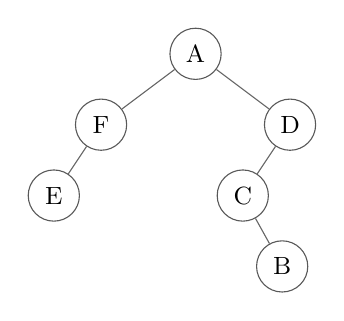
\begin{tikzpicture}[
    btn/.style={circle, draw=black!65, line width=0.4pt, minimum size=6.5mm, inner sep=0pt, font=\small},
    level distance=9mm, edge from parent/.style={draw=black!60},
    level 1/.style={sibling distance=24mm}, level 2/.style={sibling distance=12mm},
    level 3/.style={sibling distance=10mm}]
\node[btn] {A}
    child {node[btn] {F} child {node[btn] {E}} child[missing]}
    child {node[btn] {D}
        child {node[btn] {C} child[missing] child {node[btn] {B}}}
        child[missing]};
\end{tikzpicture}
\end{center}
前序（根、左、右）：A，左子樹 F E，右子樹 D C B，得到 A F E D C B，選 a)。 檢查：這棵樹的中序是
E F A C B D、後序是 E F B C D A，都和題目相同。 其他選項：b) 把 E、F 的上下弄反；c)、d) 右子樹
的根不是 D，後序都對不上。
\end{pastsoln}
